\documentclass[]{article}
\usepackage{lmodern}
\usepackage{amssymb,amsmath}
\usepackage{ifxetex,ifluatex}
\usepackage{fixltx2e} % provides \textsubscript
\ifnum 0\ifxetex 1\fi\ifluatex 1\fi=0 % if pdftex
  \usepackage[T1]{fontenc}
  \usepackage[utf8]{inputenc}
\else % if luatex or xelatex
  \ifxetex
    \usepackage{mathspec}
  \else
    \usepackage{fontspec}
  \fi
  \defaultfontfeatures{Ligatures=TeX,Scale=MatchLowercase}
\fi
% use upquote if available, for straight quotes in verbatim environments
\IfFileExists{upquote.sty}{\usepackage{upquote}}{}
% use microtype if available
\IfFileExists{microtype.sty}{%
\usepackage{microtype}
\UseMicrotypeSet[protrusion]{basicmath} % disable protrusion for tt fonts
}{}
\usepackage[margin=1in]{geometry}
\usepackage{hyperref}
\hypersetup{unicode=true,
            pdftitle={Homework 4},
            pdfauthor={Xinyi Lin},
            pdfborder={0 0 0},
            breaklinks=true}
\urlstyle{same}  % don't use monospace font for urls
\usepackage{color}
\usepackage{fancyvrb}
\newcommand{\VerbBar}{|}
\newcommand{\VERB}{\Verb[commandchars=\\\{\}]}
\DefineVerbatimEnvironment{Highlighting}{Verbatim}{commandchars=\\\{\}}
% Add ',fontsize=\small' for more characters per line
\usepackage{framed}
\definecolor{shadecolor}{RGB}{248,248,248}
\newenvironment{Shaded}{\begin{snugshade}}{\end{snugshade}}
\newcommand{\KeywordTok}[1]{\textcolor[rgb]{0.13,0.29,0.53}{\textbf{#1}}}
\newcommand{\DataTypeTok}[1]{\textcolor[rgb]{0.13,0.29,0.53}{#1}}
\newcommand{\DecValTok}[1]{\textcolor[rgb]{0.00,0.00,0.81}{#1}}
\newcommand{\BaseNTok}[1]{\textcolor[rgb]{0.00,0.00,0.81}{#1}}
\newcommand{\FloatTok}[1]{\textcolor[rgb]{0.00,0.00,0.81}{#1}}
\newcommand{\ConstantTok}[1]{\textcolor[rgb]{0.00,0.00,0.00}{#1}}
\newcommand{\CharTok}[1]{\textcolor[rgb]{0.31,0.60,0.02}{#1}}
\newcommand{\SpecialCharTok}[1]{\textcolor[rgb]{0.00,0.00,0.00}{#1}}
\newcommand{\StringTok}[1]{\textcolor[rgb]{0.31,0.60,0.02}{#1}}
\newcommand{\VerbatimStringTok}[1]{\textcolor[rgb]{0.31,0.60,0.02}{#1}}
\newcommand{\SpecialStringTok}[1]{\textcolor[rgb]{0.31,0.60,0.02}{#1}}
\newcommand{\ImportTok}[1]{#1}
\newcommand{\CommentTok}[1]{\textcolor[rgb]{0.56,0.35,0.01}{\textit{#1}}}
\newcommand{\DocumentationTok}[1]{\textcolor[rgb]{0.56,0.35,0.01}{\textbf{\textit{#1}}}}
\newcommand{\AnnotationTok}[1]{\textcolor[rgb]{0.56,0.35,0.01}{\textbf{\textit{#1}}}}
\newcommand{\CommentVarTok}[1]{\textcolor[rgb]{0.56,0.35,0.01}{\textbf{\textit{#1}}}}
\newcommand{\OtherTok}[1]{\textcolor[rgb]{0.56,0.35,0.01}{#1}}
\newcommand{\FunctionTok}[1]{\textcolor[rgb]{0.00,0.00,0.00}{#1}}
\newcommand{\VariableTok}[1]{\textcolor[rgb]{0.00,0.00,0.00}{#1}}
\newcommand{\ControlFlowTok}[1]{\textcolor[rgb]{0.13,0.29,0.53}{\textbf{#1}}}
\newcommand{\OperatorTok}[1]{\textcolor[rgb]{0.81,0.36,0.00}{\textbf{#1}}}
\newcommand{\BuiltInTok}[1]{#1}
\newcommand{\ExtensionTok}[1]{#1}
\newcommand{\PreprocessorTok}[1]{\textcolor[rgb]{0.56,0.35,0.01}{\textit{#1}}}
\newcommand{\AttributeTok}[1]{\textcolor[rgb]{0.77,0.63,0.00}{#1}}
\newcommand{\RegionMarkerTok}[1]{#1}
\newcommand{\InformationTok}[1]{\textcolor[rgb]{0.56,0.35,0.01}{\textbf{\textit{#1}}}}
\newcommand{\WarningTok}[1]{\textcolor[rgb]{0.56,0.35,0.01}{\textbf{\textit{#1}}}}
\newcommand{\AlertTok}[1]{\textcolor[rgb]{0.94,0.16,0.16}{#1}}
\newcommand{\ErrorTok}[1]{\textcolor[rgb]{0.64,0.00,0.00}{\textbf{#1}}}
\newcommand{\NormalTok}[1]{#1}
\usepackage{graphicx,grffile}
\makeatletter
\def\maxwidth{\ifdim\Gin@nat@width>\linewidth\linewidth\else\Gin@nat@width\fi}
\def\maxheight{\ifdim\Gin@nat@height>\textheight\textheight\else\Gin@nat@height\fi}
\makeatother
% Scale images if necessary, so that they will not overflow the page
% margins by default, and it is still possible to overwrite the defaults
% using explicit options in \includegraphics[width, height, ...]{}
\setkeys{Gin}{width=\maxwidth,height=\maxheight,keepaspectratio}
\IfFileExists{parskip.sty}{%
\usepackage{parskip}
}{% else
\setlength{\parindent}{0pt}
\setlength{\parskip}{6pt plus 2pt minus 1pt}
}
\setlength{\emergencystretch}{3em}  % prevent overfull lines
\providecommand{\tightlist}{%
  \setlength{\itemsep}{0pt}\setlength{\parskip}{0pt}}
\setcounter{secnumdepth}{0}
% Redefines (sub)paragraphs to behave more like sections
\ifx\paragraph\undefined\else
\let\oldparagraph\paragraph
\renewcommand{\paragraph}[1]{\oldparagraph{#1}\mbox{}}
\fi
\ifx\subparagraph\undefined\else
\let\oldsubparagraph\subparagraph
\renewcommand{\subparagraph}[1]{\oldsubparagraph{#1}\mbox{}}
\fi

%%% Use protect on footnotes to avoid problems with footnotes in titles
\let\rmarkdownfootnote\footnote%
\def\footnote{\protect\rmarkdownfootnote}

%%% Change title format to be more compact
\usepackage{titling}

% Create subtitle command for use in maketitle
\newcommand{\subtitle}[1]{
  \posttitle{
    \begin{center}\large#1\end{center}
    }
}

\setlength{\droptitle}{-2em}

  \title{Homework 4}
    \pretitle{\vspace{\droptitle}\centering\huge}
  \posttitle{\par}
    \author{Xinyi Lin}
    \preauthor{\centering\large\emph}
  \postauthor{\par}
      \predate{\centering\large\emph}
  \postdate{\par}
    \date{11/9/2018}


\begin{document}
\maketitle

\section{Problem 1}\label{problem-1}

\subsection{Question 1}\label{question-1}

\[ b_1 = \frac{n\sum x_iY_i-\sum x_i\sum Y_i}{n\sum x^2_i-(\sum x_i)^2} = \frac{\sum x_iY_i-n\hat{Y}\bar{x}}{\sum x_i^2 - n\bar{x}^2} \]

\[ b_0 = \hat{Y} - b_1 \bar{x} \] Since

\[ \sum x_iY_i - n\bar{Y}\bar{x} = \sum x_iY_i-\bar{x}\sum Y_i = \sum(x_i-\bar{x})Y_i \]

The expectation of \(b_1\)'s numerator is

\[
\begin{split}
E\{\sum (x_i-\bar{x})Y_i\} & =\sum (x_i-\bar{x})E(Y_i)\\
& =\sum(x_i - \bar{x})(\beta_0+\beta_1x_i)\\
& =\beta_0\sum x_i-n\bar{x}\beta_0+\beta_1\sum{x_i}^2-n\bar{x}^2\beta_1\\
& =\beta_1(\sum{x_i^2}-n\bar{x}^2)
\end{split} 
\]

\begin{split}
E(b_1) &=\frac{E\{\sum{(x_i-\bar{x})Y_i}\}}{\sum{x_i^2}-n\bar{x}^2}\\
&=\frac{\beta_1(\sum{x_i^2}-n\bar{x}^2)}{\sum{x_i^2}-n\bar{x}^2}\\
&=\beta_1\\

E(b_0) &= E(\hat{Y}-b_1\bar{x})\\
&=\frac{1}{n}\sum{E(Y_i)}-E(b_1)\bar{x}\\
&=\frac{1}{n}\sum{[\beta_0+\beta_1x_1]}-\beta_1\bar{x}\\
&=\frac{1}{n}[n\beta_0+n\beta_1\bar{x}]-\beta_1\bar{x}\\
&=\beta_0
\end{split}

So \(b_1\) and \(b_0\) are unbiased estimators of \(\beta_1\) and
\(\beta_0\).

\subsection{Question 2}\label{question-2}

As \(\hat{\beta_0}=\bar{Y}-\hat{\beta_1}\),
\(b_1 = \frac{n\sum x_iY_i-\sum x_i\sum Y_i}{n\sum x^2_i-(\sum x_i)^2} = \frac{\sum x_iY_i-n\hat{Y}\bar{x}}{\sum x_i^2 - n\bar{x}^2}\)
and estimated regression model
\(\hat{Y_i}=\hat{\beta_0}+\hat{\beta_1}x_i\),

when \(x_i=\bar{x}\),

\[\hat{Y_i}=\bar{Y}-\hat{\beta_1}\bar{x}+\hat{\beta_1}\bar{x}=\bar{Y}\]
so regression model always goes through the point \((\bar{x},\bar{y})\).

\subsection{Question 3}\label{question-3}

The regression model is:

\[ Yi \sim N(\beta_0 + \beta_1x_i, \sigma^2), i=1, 2, ..., n \]

the likelihood of the linear model becomes:

\[ L(\beta_0, \beta, \sigma^2) = \prod_{i=1}^n\frac{1}{\sqrt{2x\sigma}}exp(-\frac{(Y_i-\beta_0-\beta_1x_i)^2}{2\sigma^2}) \]

the log-likelihood function:

\[ lnL(\beta_0, \beta_1, \sigma^2) = log[\prod_{i=1}^n\frac{1}{\sqrt{2x\sigma}}exp(-\frac{(Y_i-\beta_0-\beta_1x_i)^2}{2\sigma^2})] = -\frac{n}{2}log(2\pi)-nlog(\sigma)-\sum_{i=1}^n\frac{(Y_i -\beta_0-\beta_1x_i)^2}{2\sigma^2} \]

to find \(\sigma\), we let

\[ \frac{\partial{lnL(\beta_0, \beta_1, \sigma^2)}}{\partial{\sigma}}= -\frac{n}{\sigma}+\frac{1}{\sigma^3}\sum_{i=1}^n(Y_i-\beta_0-\beta_1x_i)^2=0 \]

\[ \sigma^2 = \frac{1}{n}\sum_{i=1}^n(Y_i-\beta_0-\beta_1x_i)^2 \]

so estimator of \(\sigma^2\)

\[  \hat{\sigma^2} = \frac{1}{n}\sum_{i=1}^n(\hat{Y_i}-\hat{\beta_0}-\hat{\beta_1}x_i)^2 = \frac{1}{n}\sum_{i=1}^n(Y_i-\hat{Y_i})^2 = \frac{1}{n}SSE\]

\[ E(\hat{\sigma^2}) = E(\frac{1}{n}\sum_{i=1}^n(Y_i-\hat{Y})^2) = E(\frac{1}{n}SSE) = E(\frac{n-2}{n}\frac{SSE}{n-2}) = \frac{n-2}{n}E(\frac{SSE}{n-2}) = \frac{n-2}{n}\sigma^2 \]

since\(E(\hat{\sigma^2}) \neq \sigma^2\), \(\hat{\sigma^2}\) is biased
estimator of \(\sigma^2\), while
\(E(s^2) = E(\hat{\frac{SSE}{n-2}}) = \sigma^2\), \(s^2\) is unbiased
estimator of \(\sigma^2\).

\begin{Shaded}
\begin{Highlighting}[]
\KeywordTok{library}\NormalTok{(tidyverse)}
\KeywordTok{library}\NormalTok{(patchwork)}
\end{Highlighting}
\end{Shaded}

\section{Problem 2}\label{problem-2}

First, we need to import data

\begin{Shaded}
\begin{Highlighting}[]
\NormalTok{HeartDisease_df =}\StringTok{ }\KeywordTok{read_csv}\NormalTok{(}\StringTok{"./data/HeartDisease.csv"}\NormalTok{) }
\end{Highlighting}
\end{Shaded}

\begin{verbatim}
## Parsed with column specification:
## cols(
##   id = col_integer(),
##   totalcost = col_double(),
##   age = col_integer(),
##   gender = col_integer(),
##   interventions = col_integer(),
##   drugs = col_integer(),
##   ERvisits = col_integer(),
##   complications = col_integer(),
##   comorbidities = col_integer(),
##   duration = col_integer()
## )
\end{verbatim}

\begin{Shaded}
\begin{Highlighting}[]
\KeywordTok{head}\NormalTok{(HeartDisease_df)}
\end{Highlighting}
\end{Shaded}

\begin{verbatim}
## # A tibble: 6 x 10
##      id totalcost   age gender interventions drugs ERvisits complications
##   <int>     <dbl> <int>  <int>         <int> <int>    <int>         <int>
## 1     1      179.    63      0             2     1        4             0
## 2     2      319     59      0             2     0        6             0
## 3     3     9311.    62      0            17     0        2             0
## 4     4      281.    60      1             9     0        7             0
## 5     5    18727.    55      0             5     2        7             0
## 6     6      453.    66      0             1     0        3             0
## # ... with 2 more variables: comorbidities <int>, duration <int>
\end{verbatim}

\subsection{Question 1}\label{question-1-1}

This dataset includes 788 observations and 10 variables. Among
variables, main outcome is \texttt{totalcost}, main predictor is
\texttt{ERvisits} and other important covariates including \texttt{age},
\texttt{gender} and \texttt{duration}.

Then, we show descriptive statistics for all variables of interest.

\begin{Shaded}
\begin{Highlighting}[]
\NormalTok{mean_and_sd =}\StringTok{ }\ControlFlowTok{function}\NormalTok{(x) \{}
  
  \ControlFlowTok{if}\NormalTok{ (}\OperatorTok{!}\KeywordTok{is.numeric}\NormalTok{(x)) \{}
    \KeywordTok{stop}\NormalTok{(}\StringTok{"Argument x should be numeric"}\NormalTok{)}
\NormalTok{  \} }\ControlFlowTok{else} \ControlFlowTok{if}\NormalTok{ (}\KeywordTok{length}\NormalTok{(x) }\OperatorTok{==}\StringTok{ }\DecValTok{1}\NormalTok{) \{}
    \KeywordTok{stop}\NormalTok{(}\StringTok{"Cannot be computed for length 1 vectors"}\NormalTok{)}
\NormalTok{  \}}
  
\NormalTok{  mean_x =}\StringTok{ }\KeywordTok{mean}\NormalTok{(x)}
\NormalTok{  sd_x =}\StringTok{ }\KeywordTok{sd}\NormalTok{(x)}

  \KeywordTok{list}\NormalTok{(}\DataTypeTok{mean =}\NormalTok{ mean_x, }
       \DataTypeTok{sd =}\NormalTok{ sd_x)}
\NormalTok{\}}
\end{Highlighting}
\end{Shaded}

\texttt{totalcost}

\begin{Shaded}
\begin{Highlighting}[]
\KeywordTok{mean_and_sd}\NormalTok{(HeartDisease_df}\OperatorTok{$}\NormalTok{totalcost)}
\end{Highlighting}
\end{Shaded}

\begin{verbatim}
## $mean
## [1] 2799.956
## 
## $sd
## [1] 6690.26
\end{verbatim}

\texttt{ERvisits}

\begin{Shaded}
\begin{Highlighting}[]
\KeywordTok{mean_and_sd}\NormalTok{(HeartDisease_df}\OperatorTok{$}\NormalTok{ERvisits)}
\end{Highlighting}
\end{Shaded}

\begin{verbatim}
## $mean
## [1] 3.425127
## 
## $sd
## [1] 2.637474
\end{verbatim}

\texttt{age}

\begin{Shaded}
\begin{Highlighting}[]
\KeywordTok{mean_and_sd}\NormalTok{(HeartDisease_df}\OperatorTok{$}\NormalTok{age)}
\end{Highlighting}
\end{Shaded}

\begin{verbatim}
## $mean
## [1] 58.71827
## 
## $sd
## [1] 6.754118
\end{verbatim}

\texttt{gender}

\begin{Shaded}
\begin{Highlighting}[]
\KeywordTok{summary}\NormalTok{(}\KeywordTok{as.factor}\NormalTok{(HeartDisease_df}\OperatorTok{$}\NormalTok{gender))}
\end{Highlighting}
\end{Shaded}

\begin{verbatim}
##   0   1 
## 608 180
\end{verbatim}

\texttt{complications}

\begin{Shaded}
\begin{Highlighting}[]
\KeywordTok{summary}\NormalTok{(}\KeywordTok{as.factor}\NormalTok{(HeartDisease_df}\OperatorTok{$}\NormalTok{complications))}
\end{Highlighting}
\end{Shaded}

\begin{verbatim}
##   0   1   3 
## 745  42   1
\end{verbatim}

\subsection{Question 2}\label{question-2-1}

\begin{Shaded}
\begin{Highlighting}[]
\NormalTok{total_plot =}
\StringTok{  }\NormalTok{HeartDisease_df }\OperatorTok\StringTok{ }
\StringTok{  }\KeywordTok{ggplot}\NormalTok{(}\KeywordTok{aes}\NormalTok{(}\DataTypeTok{x =}\NormalTok{ totalcost)) }\OperatorTok{+}
\StringTok{  }\KeywordTok{geom_density}\NormalTok{() }\OperatorTok{+}
\StringTok{  }\KeywordTok{labs}\NormalTok{(}\DataTypeTok{title =} \StringTok{"pdf of total cost"}\NormalTok{)}
\end{Highlighting}
\end{Shaded}

\begin{Shaded}
\begin{Highlighting}[]
\NormalTok{log_plot =}\StringTok{ }
\StringTok{  }\NormalTok{HeartDisease_df }\OperatorTok\StringTok{ }
\StringTok{  }\KeywordTok{ggplot}\NormalTok{(}\KeywordTok{aes}\NormalTok{(}\DataTypeTok{x =} \KeywordTok{log}\NormalTok{(totalcost))) }\OperatorTok{+}
\StringTok{  }\KeywordTok{geom_density}\NormalTok{() }\OperatorTok{+}
\StringTok{  }\KeywordTok{labs}\NormalTok{(}\DataTypeTok{title =} \StringTok{"pdf of log(total cost)"}\NormalTok{)}
\end{Highlighting}
\end{Shaded}

\begin{Shaded}
\begin{Highlighting}[]
\NormalTok{sqrt_plot =}\StringTok{ }
\StringTok{  }\NormalTok{HeartDisease_df }\OperatorTok\StringTok{ }
\StringTok{  }\KeywordTok{ggplot}\NormalTok{(}\KeywordTok{aes}\NormalTok{(}\DataTypeTok{x =} \KeywordTok{sqrt}\NormalTok{(totalcost))) }\OperatorTok{+}
\StringTok{  }\KeywordTok{geom_density}\NormalTok{() }\OperatorTok{+}
\StringTok{  }\KeywordTok{labs}\NormalTok{(}\DataTypeTok{title =} \StringTok{"pdf of square root of total cost"}\NormalTok{)}
\end{Highlighting}
\end{Shaded}

\begin{Shaded}
\begin{Highlighting}[]
\NormalTok{square_plot =}\StringTok{ }
\StringTok{  }\NormalTok{HeartDisease_df }\OperatorTok\StringTok{ }
\StringTok{  }\KeywordTok{ggplot}\NormalTok{(}\KeywordTok{aes}\NormalTok{(}\DataTypeTok{x =}\NormalTok{ totalcost}\OperatorTok{^}\DecValTok{2}\NormalTok{)) }\OperatorTok{+}
\StringTok{  }\KeywordTok{geom_density}\NormalTok{() }\OperatorTok{+}
\StringTok{  }\KeywordTok{labs}\NormalTok{(}\DataTypeTok{title =} \StringTok{"pdf of total cost square"}\NormalTok{)}
\end{Highlighting}
\end{Shaded}

\begin{Shaded}
\begin{Highlighting}[]
\NormalTok{(total_plot }\OperatorTok{+}\StringTok{ }\NormalTok{square_plot)}\OperatorTok{/}\NormalTok{(log_plot }\OperatorTok{+}\StringTok{ }\NormalTok{sqrt_plot)}
\end{Highlighting}
\end{Shaded}

\begin{verbatim}
## Warning: Removed 3 rows containing non-finite values (stat_density).
\end{verbatim}

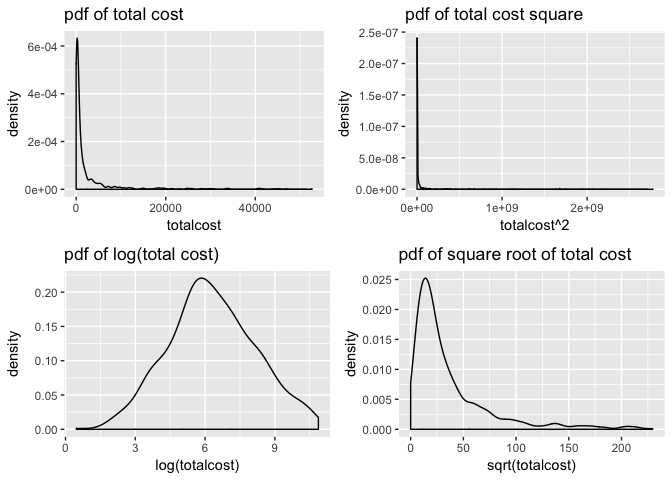
\includegraphics{HW4_xl2836_files/figure-latex/unnamed-chunk-13-1.pdf}

Above are distribution of total cost, log(totalcost), suqre root of
totalcost and totalcost square. We can find that apply log to total cost
is the best transformations.

\subsection{Question 3}\label{question-3-1}

\begin{Shaded}
\begin{Highlighting}[]
\NormalTok{HeartDisease_df =}
\StringTok{  }\NormalTok{HeartDisease_df }\OperatorTok\StringTok{ }
\StringTok{  }\KeywordTok{mutate}\NormalTok{(}\DataTypeTok{comp_bin =} \KeywordTok{ifelse}\NormalTok{(complications }\OperatorTok{==}\StringTok{ }\DecValTok{0}\NormalTok{, }\DecValTok{0}\NormalTok{, }\DecValTok{1}\NormalTok{)) }\OperatorTok\StringTok{ }
\StringTok{  }\KeywordTok{mutate}\NormalTok{(}\DataTypeTok{totalcost =} \KeywordTok{ifelse}\NormalTok{(totalcost }\OperatorTok{==}\StringTok{ }\DecValTok{0}\NormalTok{, }\FloatTok{0.001}\NormalTok{, totalcost))}

\KeywordTok{head}\NormalTok{(HeartDisease_df)}
\end{Highlighting}
\end{Shaded}

\begin{verbatim}
## # A tibble: 6 x 11
##      id totalcost   age gender interventions drugs ERvisits complications
##   <int>     <dbl> <int>  <int>         <int> <int>    <int>         <int>
## 1     1      179.    63      0             2     1        4             0
## 2     2      319     59      0             2     0        6             0
## 3     3     9311.    62      0            17     0        2             0
## 4     4      281.    60      1             9     0        7             0
## 5     5    18727.    55      0             5     2        7             0
## 6     6      453.    66      0             1     0        3             0
## # ... with 3 more variables: comorbidities <int>, duration <int>,
## #   comp_bin <dbl>
\end{verbatim}

\subsection{Question 4}\label{question-4}

\begin{Shaded}
\begin{Highlighting}[]
\NormalTok{HeartDisease_df }\OperatorTok\StringTok{ }
\StringTok{  }\KeywordTok{mutate}\NormalTok{(}\DataTypeTok{log_totalcost =} \KeywordTok{log}\NormalTok{(totalcost)) }\OperatorTok\StringTok{ }
\StringTok{  }\KeywordTok{ggplot}\NormalTok{(}\KeywordTok{aes}\NormalTok{(}\DataTypeTok{x =}\NormalTok{ log_totalcost, }\DataTypeTok{y =}\NormalTok{ ERvisits)) }\OperatorTok{+}
\StringTok{  }\KeywordTok{geom_point}\NormalTok{() }\OperatorTok{+}
\StringTok{  }\KeywordTok{geom_smooth}\NormalTok{(}\DataTypeTok{method =} \StringTok{'lm'}\NormalTok{,}\DataTypeTok{formula =}\NormalTok{ y}\OperatorTok{~}\NormalTok{x)}
\end{Highlighting}
\end{Shaded}

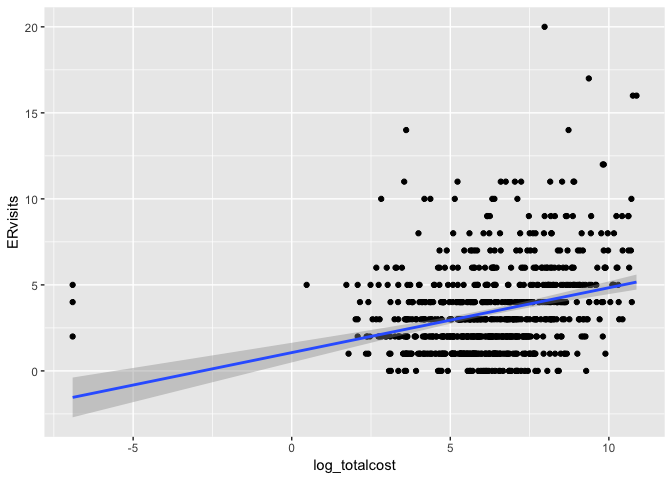
\includegraphics{HW4_xl2836_files/figure-latex/unnamed-chunk-15-1.pdf}

\begin{Shaded}
\begin{Highlighting}[]
\NormalTok{reg_Heart =}\StringTok{ }
\StringTok{  }\NormalTok{HeartDisease_df }\OperatorTok\StringTok{ }
\StringTok{  }\KeywordTok{mutate}\NormalTok{(}\DataTypeTok{log_totalcost =} \KeywordTok{log}\NormalTok{(totalcost)) }\OperatorTok\StringTok{ }
\StringTok{  }\CommentTok{#filter(is.finite(log_totalcost)) %>% }
\StringTok{  }\KeywordTok{lm}\NormalTok{(}\DataTypeTok{formula =}\NormalTok{ log_totalcost }\OperatorTok{~}\StringTok{ }\NormalTok{ERvisits, }\DataTypeTok{data =}\NormalTok{ .) }

\NormalTok{reg_Heart }\OperatorTok\StringTok{ }
\StringTok{  }\NormalTok{broom}\OperatorTok{::}\KeywordTok{tidy}\NormalTok{()}
\end{Highlighting}
\end{Shaded}

\begin{verbatim}
## # A tibble: 2 x 5
##   term        estimate std.error statistic   p.value
##   <chr>          <dbl>     <dbl>     <dbl>     <dbl>
## 1 (Intercept)    5.49     0.114      48.2  3.56e-237
## 2 ERvisits       0.225    0.0263      8.53 7.39e- 17
\end{verbatim}

\begin{Shaded}
\begin{Highlighting}[]
\KeywordTok{summary}\NormalTok{(reg_Heart)}
\end{Highlighting}
\end{Shaded}

\begin{verbatim}
## 
## Call:
## lm(formula = log_totalcost ~ ERvisits, data = .)
## 
## Residuals:
##      Min       1Q   Median       3Q      Max 
## -13.5255  -1.0922   0.0608   1.3147   4.3314 
## 
## Coefficients:
##             Estimate Std. Error t value Pr(>|t|)    
## (Intercept)  5.49384    0.11387  48.248   <2e-16 ***
## ERvisits     0.22477    0.02635   8.531   <2e-16 ***
## ---
## Signif. codes:  0 '***' 0.001 '**' 0.01 '*' 0.05 '.' 0.1 ' ' 1
## 
## Residual standard error: 1.949 on 786 degrees of freedom
## Multiple R-squared:  0.08475,    Adjusted R-squared:  0.08359 
## F-statistic: 72.78 on 1 and 786 DF,  p-value: < 2.2e-16
\end{verbatim}

According to the results, we can find that adjusted R-squared is 0.1014
which is very closed to 0 and means this simple linear model is not a
proper model. However, p-value of slope is lower than 2.2e-16, which
means the slope is significant and there are positive relationship
between log of total cost and number of emergency room visits.

Interpretation: The slop of model is 0.227 which means if the number of
emergency room vistis increases by 1 unit, the log of total cost will
increase 0.452 units.

\subsection{Question 5}\label{question-5}

Test if \texttt{comp\_bin} is an effect modifier

\begin{Shaded}
\begin{Highlighting}[]
\NormalTok{reg_modifier_Heart =}\StringTok{ }
\StringTok{  }\NormalTok{HeartDisease_df }\OperatorTok\StringTok{ }
\StringTok{  }\KeywordTok{mutate}\NormalTok{(}\DataTypeTok{log_totalcost =} \KeywordTok{log}\NormalTok{(totalcost)) }\OperatorTok\StringTok{ }
\StringTok{  }\CommentTok{#filter(is.finite(log_totalcost)) %>% }
\StringTok{  }\KeywordTok{lm}\NormalTok{(}\DataTypeTok{formula =}\NormalTok{ log_totalcost }\OperatorTok{~}\StringTok{ }\NormalTok{ERvisits }\OperatorTok{+}\StringTok{ }\NormalTok{comp_bin }\OperatorTok{+}\StringTok{ }\NormalTok{ERvisits}\OperatorTok{*}\NormalTok{comp_bin, }\DataTypeTok{data =}\NormalTok{ .) }

\NormalTok{reg_modifier_Heart }\OperatorTok\StringTok{ }
\StringTok{  }\NormalTok{broom}\OperatorTok{::}\KeywordTok{tidy}\NormalTok{()}
\end{Highlighting}
\end{Shaded}

\begin{verbatim}
## # A tibble: 4 x 5
##   term              estimate std.error statistic   p.value
##   <chr>                <dbl>     <dbl>     <dbl>     <dbl>
## 1 (Intercept)         5.46      0.114     47.8   1.12e-234
## 2 ERvisits            0.208     0.0271     7.70  4.01e- 14
## 3 comp_bin            2.22      0.602      3.69  2.39e-  4
## 4 ERvisits:comp_bin  -0.0964    0.105     -0.921 3.57e-  1
\end{verbatim}

\begin{Shaded}
\begin{Highlighting}[]
\KeywordTok{summary}\NormalTok{(reg_modifier_Heart)}
\end{Highlighting}
\end{Shaded}

\begin{verbatim}
## 
## Call:
## lm(formula = log_totalcost ~ ERvisits + comp_bin + ERvisits * 
##     comp_bin, data = .)
## 
## Residuals:
##      Min       1Q   Median       3Q      Max 
## -13.4051  -1.0559   0.0325   1.2269   4.4353 
## 
## Coefficients:
##                   Estimate Std. Error t value Pr(>|t|)    
## (Intercept)        5.45548    0.11406  47.828  < 2e-16 ***
## ERvisits           0.20837    0.02705   7.703 4.01e-14 ***
## comp_bin           2.22320    0.60233   3.691 0.000239 ***
## ERvisits:comp_bin -0.09639    0.10461  -0.921 0.357103    
## ---
## Signif. codes:  0 '***' 0.001 '**' 0.01 '*' 0.05 '.' 0.1 ' ' 1
## 
## Residual standard error: 1.911 on 784 degrees of freedom
## Multiple R-squared:  0.1227, Adjusted R-squared:  0.1193 
## F-statistic: 36.55 on 3 and 784 DF,  p-value: < 2.2e-16
\end{verbatim}

Since the corresponding p-value of 'ERvisits*comp\_bin' is 0.357 which
is bigger than 0.05, we can conclude that there is no interaction
between \texttt{ERvisits} and \texttt{comp\_bin} and \texttt{comp\_bin}
is not a modifier.

Test if \texttt{comp\_bin} is a confunder.

\begin{Shaded}
\begin{Highlighting}[]
\NormalTok{reg_confounder_Heart =}\StringTok{ }
\StringTok{  }\NormalTok{HeartDisease_df }\OperatorTok\StringTok{ }
\StringTok{  }\KeywordTok{mutate}\NormalTok{(}\DataTypeTok{log_totalcost =} \KeywordTok{log}\NormalTok{(totalcost)) }\OperatorTok\StringTok{ }
\StringTok{  }\CommentTok{#filter(is.finite(log_totalcost)) %>% }
\StringTok{  }\KeywordTok{lm}\NormalTok{(}\DataTypeTok{formula =}\NormalTok{ log_totalcost }\OperatorTok{~}\StringTok{ }\NormalTok{ERvisits }\OperatorTok{+}\StringTok{ }\NormalTok{comp_bin, }\DataTypeTok{data =}\NormalTok{ .) }

\NormalTok{reg_confounder_Heart }\OperatorTok\StringTok{ }
\StringTok{  }\NormalTok{broom}\OperatorTok{::}\KeywordTok{tidy}\NormalTok{()}
\end{Highlighting}
\end{Shaded}

\begin{verbatim}
## # A tibble: 3 x 5
##   term        estimate std.error statistic   p.value
##   <chr>          <dbl>     <dbl>     <dbl>     <dbl>
## 1 (Intercept)    5.48     0.112      49.1  2.79e-241
## 2 ERvisits       0.202    0.0261      7.73 3.33e- 14
## 3 comp_bin       1.74     0.303       5.75 1.27e-  8
\end{verbatim}

\begin{Shaded}
\begin{Highlighting}[]
\KeywordTok{summary}\NormalTok{(reg_confounder_Heart)}
\end{Highlighting}
\end{Shaded}

\begin{verbatim}
## 
## Call:
## lm(formula = log_totalcost ~ ERvisits + comp_bin, data = .)
## 
## Residuals:
##      Min       1Q   Median       3Q      Max 
## -13.3943  -1.0451   0.0252   1.2191   4.4397 
## 
## Coefficients:
##             Estimate Std. Error t value Pr(>|t|)    
## (Intercept)  5.47693    0.11165  49.054  < 2e-16 ***
## ERvisits     0.20193    0.02613   7.728 3.33e-14 ***
## comp_bin     1.74365    0.30321   5.751 1.27e-08 ***
## ---
## Signif. codes:  0 '***' 0.001 '**' 0.01 '*' 0.05 '.' 0.1 ' ' 1
## 
## Residual standard error: 1.911 on 785 degrees of freedom
## Multiple R-squared:  0.1218, Adjusted R-squared:  0.1195 
## F-statistic: 54.41 on 2 and 785 DF,  p-value: < 2.2e-16
\end{verbatim}

When adding \texttt{comp\_bin} in model the association between
\texttt{log\_totalcost} and \texttt{ERvisits} becomes smaller but still
significant and the regression coefficient decreased by 10.2\%, so
\texttt{comp\_bin} is a confounder.

Since \texttt{comp\_bin} is a confounder but not a modifier, we use
`Partial' F-test to test whether we should include \texttt{comp\_bin} as
a factor.

Model 1:
\(Y_i = \beta_0 + \beta_1X_{i1} + \beta_2X_{i2} + \varepsilon_i\)

Model 2: \(Y_i = \beta_0 + \beta_1X_{i1} + \varepsilon_i\)

Among which, \(X_1\) represents \texttt{ER\_visits}, \(X_2\) represents
\texttt{comp\_bin}.

Null hypothesis \(H_O: \beta_2 = 0\), alternative hypothesis
\(H_1: \beta_2 \neq 0\)

Decision rule:

\[ F^*=\frac{(SSR_L-SSR_S)/(df_L-df_S)}{\frac{SSE_L}{df_L}} \sim F_{df_L-df_S,dfL} \]

where \(df_S = n-p_S-1, df_L = n-p_L-1\).

If \(F^* > F(1-\alpha;df_L-df_S,df_L)\), reject \(H_0\);

If \(F^* \leq F(1-\alpha;df_L-df_S,df_L)\), fail to reject \(H_0\).

With \(\alpha = 0.05\), when \(p-value \geq 0.05\), fail to reject
\(H_0\), when \(p-value < 0.05\), reject \(H_0\).

\begin{Shaded}
\begin{Highlighting}[]
\KeywordTok{anova}\NormalTok{(reg_confounder_Heart, reg_Heart) }\OperatorTok\StringTok{ }
\StringTok{  }\NormalTok{broom}\OperatorTok{::}\KeywordTok{tidy}\NormalTok{()}
\end{Highlighting}
\end{Shaded}

\begin{verbatim}
## Warning: Unknown or uninitialised column: 'term'.
\end{verbatim}

\begin{verbatim}
## # A tibble: 2 x 6
##   res.df   rss    df sumsq statistic       p.value
## *  <dbl> <dbl> <dbl> <dbl>     <dbl>         <dbl>
## 1    785 2866.    NA   NA       NA   NA           
## 2    786 2987.    -1 -121.      33.1  0.0000000127
\end{verbatim}

According to results, p-value is smaller than 0.01 so we reject \(H_0\)
and conclude that Model 1 is `superior'.As a resuit, we should include
\texttt{comp\_bin} should be added in the model and model 1 is
`superior'.

\subsection{Question 6}\label{question-6}

\begin{Shaded}
\begin{Highlighting}[]
\NormalTok{reg_added_Heart =}\StringTok{ }
\StringTok{  }\NormalTok{HeartDisease_df }\OperatorTok\StringTok{ }
\StringTok{  }\KeywordTok{mutate}\NormalTok{(}\DataTypeTok{log_totalcost =} \KeywordTok{log}\NormalTok{(totalcost)) }\OperatorTok\StringTok{ }
\StringTok{  }\CommentTok{#filter(is.finite(log_totalcost)) %>% }
\StringTok{  }\KeywordTok{lm}\NormalTok{(}\DataTypeTok{formula =}\NormalTok{ log_totalcost }\OperatorTok{~}\StringTok{ }\NormalTok{ERvisits }\OperatorTok{+}\StringTok{ }\NormalTok{comp_bin }\OperatorTok{+}\StringTok{ }\NormalTok{age }\OperatorTok{+}\StringTok{ }\NormalTok{gender }\OperatorTok{+}\StringTok{ }\NormalTok{duration, }\DataTypeTok{data =}\NormalTok{ .) }

\NormalTok{reg_added_Heart }\OperatorTok\StringTok{ }
\StringTok{  }\NormalTok{broom}\OperatorTok{::}\KeywordTok{tidy}\NormalTok{()}
\end{Highlighting}
\end{Shaded}

\begin{verbatim}
## # A tibble: 6 x 5
##   term        estimate std.error statistic  p.value
##   <chr>          <dbl>     <dbl>     <dbl>    <dbl>
## 1 (Intercept)  5.80     0.556        10.4  5.91e-24
## 2 ERvisits     0.173    0.0246        7.05 4.07e-12
## 3 comp_bin     1.53     0.282         5.45 6.89e- 8
## 4 age         -0.0193   0.00945      -2.05 4.10e- 2
## 5 gender      -0.323    0.151        -2.14 3.26e- 2
## 6 duration     0.00606  0.000533     11.4  6.76e-28
\end{verbatim}

\begin{Shaded}
\begin{Highlighting}[]
\KeywordTok{summary}\NormalTok{(reg_added_Heart)}
\end{Highlighting}
\end{Shaded}

\begin{verbatim}
## 
## Call:
## lm(formula = log_totalcost ~ ERvisits + comp_bin + age + gender + 
##     duration, data = .)
## 
## Residuals:
##      Min       1Q   Median       3Q      Max 
## -12.1885  -0.9962  -0.0838   1.0099   4.3499 
## 
## Coefficients:
##               Estimate Std. Error t value Pr(>|t|)    
## (Intercept)  5.8016080  0.5559910  10.435  < 2e-16 ***
## ERvisits     0.1732359  0.0245897   7.045 4.07e-12 ***
## comp_bin     1.5335773  0.2815738   5.446 6.89e-08 ***
## age         -0.0193389  0.0094493  -2.047   0.0410 *  
## gender      -0.3234418  0.1510875  -2.141   0.0326 *  
## duration     0.0060629  0.0005325  11.386  < 2e-16 ***
## ---
## Signif. codes:  0 '***' 0.001 '**' 0.01 '*' 0.05 '.' 0.1 ' ' 1
## 
## Residual standard error: 1.769 on 782 degrees of freedom
## Multiple R-squared:  0.2502, Adjusted R-squared:  0.2454 
## F-statistic: 52.18 on 5 and 782 DF,  p-value: < 2.2e-16
\end{verbatim}

According to results, we can find all p-value of covariates are smaller
than 0.01, so all covariates have significant influence in total cost.

We use `Partial' F-test to compare SLR and MLR models.

Model 1:
\(Y_i = \beta_0 + \beta_1X_{i1} + \beta_2X_{i2} + \beta_3X_{i3} + \beta_4X_{i4} + \beta_5X_{i5} + \varepsilon_i\)

Model 2: \(Y_i = \beta_0 + \beta_1X_{i1} + \varepsilon_i\)

Among which, \(X_1\) represents \texttt{ERvisits}, \(X_2\) represents
\texttt{comp\_bin}, \(X_3\) represents \texttt{age}, \(X_4\) represents
\texttt{gender}, \(X_5\) represents \texttt{duration}.

Null hypothesis \(H_O: \beta_2 = \beta_3 = \beta_4 = \beta_5 = 0\),
alternative hypothesis \(H_1:\) at least one of \(\beta\) is not zero.

Decision rule:

\[ F^*=\frac{(SSR_L-SSR_S)/(df_L-df_S)}{\frac{SSE_L}{df_L}} \sim F_{df_L-df_S,dfL} \]

where \(df_S = n-p_S-1, df_L = n-p_L-1\).

If \(F^* > F(1-\alpha;df_L-df_S,df_L)\), reject \(H_0\);

If \(F^* \leq F(1-\alpha;df_L-df_S,df_L)\), fail to reject \(H_0\).

With \(\alpha = 0.05\), when \(p-value \geq 0.05\), fail to reject
\(H_0\), when \(p-value < 0.05\), reject \(H_0\).

\begin{Shaded}
\begin{Highlighting}[]
\KeywordTok{anova}\NormalTok{(reg_Heart, reg_added_Heart) }\OperatorTok\StringTok{ }\NormalTok{broom}\OperatorTok{::}\KeywordTok{tidy}\NormalTok{()}
\end{Highlighting}
\end{Shaded}

\begin{verbatim}
## Warning: Unknown or uninitialised column: 'term'.
\end{verbatim}

\begin{verbatim}
## # A tibble: 2 x 6
##   res.df   rss    df sumsq statistic   p.value
## *  <dbl> <dbl> <dbl> <dbl>     <dbl>     <dbl>
## 1    786 2987.    NA   NA       NA   NA       
## 2    782 2447.     4  540.      43.1  1.00e-32
\end{verbatim}

According to the ANOVA results, p-value is smaller than 0.01 so we
reject \(H_0\) and conclude that Model 1 is `superior'.As a resuit, we
should use MLR model.

\section{Problem 3}\label{problem-3}

First, we import data

\begin{Shaded}
\begin{Highlighting}[]
\NormalTok{PatSatisfaction_df =}\StringTok{ }\NormalTok{readxl}\OperatorTok{::}\KeywordTok{read_xlsx}\NormalTok{(}\StringTok{"./data/PatSatisfaction.xlsx"}\NormalTok{) }\OperatorTok\StringTok{ }
\StringTok{  }\NormalTok{janitor}\OperatorTok{::}\KeywordTok{clean_names}\NormalTok{() }\OperatorTok\StringTok{ }
\StringTok{  }\NormalTok{reshape}\OperatorTok{::}\KeywordTok{rename}\NormalTok{(}\KeywordTok{c}\NormalTok{(}\DataTypeTok{safisfaction =} \StringTok{"satisfaction"}\NormalTok{))}

\KeywordTok{head}\NormalTok{(PatSatisfaction_df)}
\end{Highlighting}
\end{Shaded}

\begin{verbatim}
## # A tibble: 6 x 4
##   satisfaction   age severity anxiety
##          <dbl> <dbl>    <dbl>   <dbl>
## 1           48    50       51     2.3
## 2           57    36       46     2.3
## 3           66    40       48     2.2
## 4           70    41       44     1.8
## 5           89    28       43     1.8
## 6           36    49       54     2.9
\end{verbatim}

\subsection{Question 1}\label{question-1-2}

\begin{Shaded}
\begin{Highlighting}[]
\NormalTok{PatSatisfaction_df }\OperatorTok\StringTok{ }
\StringTok{  }\KeywordTok{cor}\NormalTok{()}
\end{Highlighting}
\end{Shaded}

\begin{verbatim}
##              satisfaction        age   severity    anxiety
## satisfaction    1.0000000 -0.7867555 -0.6029417 -0.6445910
## age            -0.7867555  1.0000000  0.5679505  0.5696775
## severity       -0.6029417  0.5679505  1.0000000  0.6705287
## anxiety        -0.6445910  0.5696775  0.6705287  1.0000000
\end{verbatim}

According to the correlation matrix, we can find that all \texttt{age},
\texttt{severity}, \texttt{anxirty} have negative relationship with
satisfaction and the relationship between \texttt{age} and
\texttt{satisfaction} is stronger than \texttt{severity} and
\texttt{anxiety} .

\subsection{Question 2}\label{question-2-2}

Assuming the model is
\[ Y_i = \beta_0 + \beta_1X_{i1} + \beta_2X_{i2} + \beta_3X_{i3} + \varepsilon_i \]
Among which, \(X_1\) represents \texttt{age}, \(X_2\) represents
\texttt{severity}, \(X_3\) represents \texttt{anxiety}.

Null hypothesis \(H_0 : \beta_1 = \beta_2 = \beta_3 =0\), alternative
hypothesis \(H_1 :\) at least one \(\beta\) is not zero.

Decision rule:

If \(F^* = \frac{MSR}{MSE} > F(1-\alpha;p,n-p-1)\), reject \(H_0\),

if \(F^* = \frac{MSR}{MSE} \leq F(1-\alpha;p,n-p-1)\), fail to reject
\(H_0\).

with a significance level of 0.05, \(\alpha = 0.05\)

\begin{Shaded}
\begin{Highlighting}[]
\NormalTok{reg_all =}\StringTok{ }
\StringTok{  }\NormalTok{PatSatisfaction_df }\OperatorTok
\StringTok{  }\KeywordTok{lm}\NormalTok{(satisfaction }\OperatorTok{~}\StringTok{ }\NormalTok{age }\OperatorTok{+}\StringTok{ }\NormalTok{severity }\OperatorTok{+}\StringTok{ }\NormalTok{anxiety, }\DataTypeTok{data =}\NormalTok{ .)}

\KeywordTok{summary}\NormalTok{(reg_all)}
\end{Highlighting}
\end{Shaded}

\begin{verbatim}
## 
## Call:
## lm(formula = satisfaction ~ age + severity + anxiety, data = .)
## 
## Residuals:
##      Min       1Q   Median       3Q      Max 
## -18.3524  -6.4230   0.5196   8.3715  17.1601 
## 
## Coefficients:
##             Estimate Std. Error t value Pr(>|t|)    
## (Intercept) 158.4913    18.1259   8.744 5.26e-11 ***
## age          -1.1416     0.2148  -5.315 3.81e-06 ***
## severity     -0.4420     0.4920  -0.898   0.3741    
## anxiety     -13.4702     7.0997  -1.897   0.0647 .  
## ---
## Signif. codes:  0 '***' 0.001 '**' 0.01 '*' 0.05 '.' 0.1 ' ' 1
## 
## Residual standard error: 10.06 on 42 degrees of freedom
## Multiple R-squared:  0.6822, Adjusted R-squared:  0.6595 
## F-statistic: 30.05 on 3 and 42 DF,  p-value: 1.542e-10
\end{verbatim}

According to results, we can find \(F^*\) = 30.05 \textgreater{}
2.8270487, so we reject \(H_0\) and conclude that there is a regression
relation.

\subsection{Question 3}\label{question-3-2}

\begin{Shaded}
\begin{Highlighting}[]
\NormalTok{reg_all }\OperatorTok\StringTok{ }\NormalTok{broom}\OperatorTok{::}\KeywordTok{tidy}\NormalTok{()}
\end{Highlighting}
\end{Shaded}

\begin{verbatim}
## # A tibble: 4 x 5
##   term        estimate std.error statistic  p.value
##   <chr>          <dbl>     <dbl>     <dbl>    <dbl>
## 1 (Intercept)  158.       18.1       8.74  5.26e-11
## 2 age           -1.14      0.215    -5.31  3.81e- 6
## 3 severity      -0.442     0.492    -0.898 3.74e- 1
## 4 anxiety      -13.5       7.10     -1.90  6.47e- 2
\end{verbatim}

\begin{Shaded}
\begin{Highlighting}[]
\KeywordTok{confint}\NormalTok{(reg_all)}
\end{Highlighting}
\end{Shaded}

\begin{verbatim}
##                  2.5 %      97.5 %
## (Intercept) 121.911727 195.0707761
## age          -1.575093  -0.7081303
## severity     -1.434831   0.5508228
## anxiety     -27.797859   0.8575324
\end{verbatim}

By using function \texttt{confint}, we get 95\% CIs of all estimators.
The 95\% CIs of \texttt{severity} is (-1.4348, 0.5508) which means at
\(\alpha = 0.05\) significant level, we can conclude that the mean value
of satisfaction changes somewhere between decreasing 1.4348 and
increasing 0.5508 for each additional unit of the severity of the
illness given all other values of predictors stay constant.

The estimated coefficient of \texttt{severity} is -0.442 which means if
the value of \texttt{severity} increased by 1 units, the mean value of
satisfaction will decrease 0.442 given all other values of predictors
stay constant.

\subsection{Question 4}\label{question-4-1}

\begin{Shaded}
\begin{Highlighting}[]
\KeywordTok{list}\NormalTok{(}\DataTypeTok{age =} \DecValTok{35}\NormalTok{, }\DataTypeTok{severity =} \DecValTok{42}\NormalTok{, }\DataTypeTok{anxiety =} \FloatTok{2.1}\NormalTok{) }\OperatorTok\StringTok{ }
\StringTok{  }\KeywordTok{predict}\NormalTok{(}\DataTypeTok{object =}\NormalTok{ reg_all, }\DataTypeTok{newdata =}\NormalTok{ ., }\DataTypeTok{interval =} \StringTok{"predict"}\NormalTok{)}
\end{Highlighting}
\end{Shaded}

\begin{verbatim}
##        fit      lwr      upr
## 1 71.68332 50.06237 93.30426
\end{verbatim}

By using \texttt{predict} function, we can get the prediction interval
for the new patient's satisfaction is (50.0624, 93.3042).

Interprest: We are 95\% confident that the the new patient's
satisfaction fall within (50.0624, 93.3042) given \texttt{age} equals
35, \texttt{severity} equals 42 and \texttt{anxiety} equals 2.1

\subsection{Question 5}\label{question-5-1}

Model 1:
\(Y_i = \beta_0 + \beta_1X_{i1} + \beta_2X_{i2} + \beta_3X_{i3} + \varepsilon_i\)

Model 2:
\(Y_i = \beta_0 + \beta_1X_{i1} + \beta_2X_{i2} + \varepsilon_i\)

Among which, \(X_1\) represents \texttt{age}, \(X_2\) represents
\texttt{severity}, \(X_3\) represents \texttt{anxiety}.

We use `Partial' F-test for nested models. Null hypothesis
\(H_O: \beta_3 = 0\), alternative hypothesis \(H_1: \beta_3 \neq 0\)

Decision rule:

\[ F^*=\frac{(SSR_L-SSR_S)/(df_L-df_S)}{\frac{SSE_L}{df_L}} \sim F_{df_L-df_S,dfL} \]

where \(df_S = n-p_S-1, df_L = n-p_L-1\).

If \(F^* > F(1-\alpha;df_L-df_S,df_L)\), reject \(H_0\);

If \(F^* \leq F(1-\alpha;df_L-df_S,df_L)\), fail to reject \(H_0\).

With \(\alpha = 0.05\), when \(p-value \geq 0.05\), fail to reject
\(H_0\), when \(p-value < 0.05\), reject \(H_0\).

\begin{Shaded}
\begin{Highlighting}[]
\NormalTok{reg_without_anxiety =}\StringTok{ }
\StringTok{  }\NormalTok{PatSatisfaction_df }\OperatorTok
\StringTok{  }\KeywordTok{lm}\NormalTok{(satisfaction }\OperatorTok{~}\StringTok{ }\NormalTok{age }\OperatorTok{+}\StringTok{ }\NormalTok{severity, }\DataTypeTok{data =}\NormalTok{ .)}

\KeywordTok{anova}\NormalTok{(reg_all, reg_without_anxiety) }\OperatorTok\StringTok{ }
\StringTok{  }\NormalTok{broom}\OperatorTok{::}\KeywordTok{tidy}\NormalTok{()}
\end{Highlighting}
\end{Shaded}

\begin{verbatim}
## Warning: Unknown or uninitialised column: 'term'.
\end{verbatim}

\begin{verbatim}
## # A tibble: 2 x 6
##   res.df   rss    df sumsq statistic p.value
## *  <dbl> <dbl> <dbl> <dbl>     <dbl>   <dbl>
## 1     42 4249.    NA   NA      NA    NA     
## 2     43 4613.    -1 -364.      3.60  0.0647
\end{verbatim}

According to the ANOVA results, p-value is 0.0647 which is larger than
0.05, so we fail to reject \(H_0\) and conclude that Model 1 is not
'superior` and we should use Model 2.


\end{document}
